\documentclass[a4paper,oneside,12pt]{extreport}

\usepackage{mmap}
\usepackage[T2A]{fontenc}
\usepackage[utf8]{inputenc}
\usepackage[english,russian]{babel}

\renewcommand{\ttdefault}{PTMono-TLF}

% Текст отчёта следует печатать, соблюдая следующие размеры полей:
% левое — 30 мм, правое — 15 мм, верхнее и нижнее — 20 мм.
\usepackage[left=20mm, right=15mm, top=15mm, bottom=15mm]{geometry}

% \setlength{\parindent}{1.25cm} % Абзацный отступ

\usepackage{setspace}
\onehalfspacing % Полуторный интервал

\frenchspacing % Равномерные пробелы
\usepackage{indentfirst} % Красная строка

\usepackage{microtype}
\sloppy

\usepackage{titlesec}
\titlespacing*{\chapter}{0pt}{-30pt}{8pt}
\titlespacing*{\section}{\parindent}{*4}{*4}
\titlespacing*{\subsection}{\parindent}{*4}{*4}
\titleformat{\chapter}{\LARGE\bfseries}{\thechapter}{20pt}{\LARGE\bfseries}
\titleformat{\section}{\Large\bfseries}{\thesection}{40pt}{\Large\bfseries}

\usepackage{graphicx}
\usepackage{caption}
\usepackage{float}

\usepackage[unicode,pdftex]{hyperref}
\hypersetup{
	hidelinks=true,
	colorlinks=true,
	linkcolor=black,
	urlcolor=blue,
}

%% title begin
\usepackage{wrapfig}

\makeatletter
	\def\vhrulefill#1{\leavevmode\leaders\hrule\@height#1\hfill \kern\z@}
\makeatother
%% title end

%% begin code
\usepackage{listings}
\usepackage{xcolor}

\lstset{
	basicstyle=\scriptsize\ttfamily,
	breakatwhitespace=true,
	breaklines=true,
	commentstyle=\color{gray},
	frame=single,
	keywordstyle=\color{blue},
	numbers=left,
	numbersep=5pt,
	numberstyle=\tiny\ttfamily\color{gray},
	showstringspaces=false,
	stringstyle=\color{red},
	tabsize=8
}

\newcommand{\code}[1]{\texttt{#1}}
%% end code

\usepackage{amsmath}
\usepackage{amssymb}
\usepackage{commath}
\usepackage{icomma}


\begin{document}

\begin{titlepage}
	{\large % 14pt instead of 12pt
	\onehalfspacing
	\centering

	\begin{wrapfigure}[7]{l}{0.14\linewidth}
		\vspace{3mm}
		\hspace{-10mm}
		
\includegraphics[width=0.93\linewidth]{inc/img/bmstu-logo}
	\end{wrapfigure}
	{\singlespacing \footnotesize \bfseries Министерство науки и высшего образования Российской Федерации\\Федеральное государственное бюджетное образовательное учреждение\\высшего образования\\<<Московский государственный технический университет\\имени Н.~Э.~Баумана\\ (национальный исследовательский университет)>>\\(МГТУ им. Н.~Э.~Баумана)\\}

	\vspace{-2.2mm}
	\vhrulefill{0.9mm}\\
	\vspace{-7.5mm}
	\vhrulefill{0.2mm}\\
	\vspace{2mm}

	{\doublespacing \small \raggedright ФАКУЛЬТЕТ \hspace{37mm} «Информатика и системы управления»\\
	КАФЕДРА \hspace{17mm} «Программное обеспечение ЭВМ и информационные технологии»\\}

	\vspace{30mm}

	\textbf{ОТЧЁТ}\\
	По лабораторной работе № 9\\
	По курсу: «Компьютерные сети»\\
	Тема: «Изучение технологии виртуальных локальных сетей (VLan) в сетевом симуляторе. Настройка маршрутизации между VLan»\\
	Вариант: 6\\

	\vspace{40mm}

	\begin{flushleft}
		\begin{tabular}{lr}
			\textbf{Студент:}        & Керимов~А.~Ш. \\
			\textbf{Группа:}         & ИУ7-74Б       \\
			\textbf{Оценка (баллы):} & \hrulefill    \\
			\textbf{Преподаватель:}  & Рогозин~Н.~О. \\
		\end{tabular}
	\end{flushleft}

	\vfill

	Москва\\
	\the\year\\}
\end{titlepage}

\setcounter{page}{2}


\tableofcontents

\chapter{Задание 1}

Назначить адреса подсетей:
\begin{enumerate}
	\item Подсеть 1: 192.168.6.0/24
	\item Подсеть 2: 192.168.7.0/24
	\item Подсеть 3: 192.168.8.0/24
	\item Подсеть 4: 192.168.9.0/24
	\item Подсеть 5 (В задаче III): 192.168.16.0/24
\end{enumerate}

\section{Настройка}

Настройка маршрутизаторов:

\begin{lstlisting}[gobble=8, caption=Настройка маршрутизатора Router0]
	Router>en
	Router#conf t
	Router(config)#in G 0/0/0
	Router(config-if)#ip ad 192.168.6.254 255.255.255.0
	Router(config-if)#ex
	Router(config)#in S 0/1/0
	Router(config-if)#ip ad 192.168.8.254 255.255.255.0
	Router(config-if)#ex
	Router(config)#ex
	Router#ex
\end{lstlisting}

\begin{lstlisting}[gobble=8, caption=Настройка маршрутизатора Router1]
	Router>en
	Router#conf t
	Router(config)#in G 0/0/0
	Router(config-if)#ip ad 192.168.7.254 255.255.255.0
	Router(config-if)#ex
	Router(config)#in S 0/1/0
	Router(config-if)#ip ad 192.168.9.254 255.255.255.0
	Router(config-if)#ex
	Router(config)#ex
	Router#ex
\end{lstlisting}

\begin{lstlisting}[gobble=8, caption=Настройка маршрутизатора Router2]
	Router>en
	Router#conf t
	Router(config)#in S 0/1/0
	Router(config-if)#ip ad 192.168.8.253 255.255.255.0
	Router(config-if)#ex
	Router(config)#in S 0/1/1
	Router(config-if)#ip ad 192.168.9.253 255.255.255.0
	Router(config-if)#ex
	Router(config)#ex
	Router#ex
\end{lstlisting}

\begin{lstlisting}[gobble=8, caption=Настройка маршрутизатора Router7]
	Router>en
	Router#conf t
	Router(config)#in G 0/0/0
	Router(config-if)#ip ad 192.168.6.254 255.255.255.0
	Router(config-if)#no sh
	Router(config-if)#ex
	Router(config)#in G 0/0/1
	Router(config-if)#ip ad 192.168.16.254 255.255.255.0
	Router(config-if)#no sh
	Router(config-if)#ex
	Router(config)#ex
	Router#ex
\end{lstlisting}

\begin{lstlisting}[gobble=8, caption=Настройка маршрутизатора Router8]
	Router>en
	Router#conf t
	Router(config)#in G 0/0/0
	Router(config-if)#ip ad 192.168.7.254 255.255.255.0
	Router(config-if)#no sh
	Router(config-if)#ex
	Router(config)#in G 0/0/1
	Router(config-if)#ip ad 192.168.16.253 255.255.255.0
	Router(config-if)#no sh
	Router(config-if)#ex
	Router(config)#ex
	Router#ex
\end{lstlisting}

\begin{lstlisting}[gobble=8, caption=Настройка маршрутизатора Router9]
	Router>en
	Router#conf t
	Router(config)#in G 0/0/0
	Router(config-if)#ip ad 192.168.8.254 255.255.255.0
	Router(config-if)#no sh
	Router(config-if)#ex
	Router(config)#in G 0/0/1
	Router(config-if)#ip ad 192.168.16.252 255.255.255.0
	Router(config-if)#no sh
	Router(config-if)#ex
	Router(config)#ex
	Router#ex
\end{lstlisting}

\begin{lstlisting}[gobble=8, caption=Настройка маршрутизатора Router10]
	Router>en
	Router#conf t
	Router(config)#in G 0/0/0
	Router(config-if)#ip ad 192.168.9.254 255.255.255.0
	Router(config-if)#no sh
	Router(config-if)#ex
	Router(config)#in G 0/0/1
	Router(config-if)#ip ad 192.168.16.251 255.255.255.0
	Router(config-if)#no sh
	Router(config-if)#ex
	Router(config)#ex
	Router#ex
\end{lstlisting}

На хостах были настроены адреса интерфейсов и адреса шлюзов по умолчанию.

\chapter{Задание 2}

Настроить динамическую маршрутизацию в прилагаемом .pkt файле на стенде I через протокол RIPv2 так, чтобы пинг любым хостом или маршрутизатором любого другого хоста или маршрутизатора был успешным.
Представить отдельным .pkt файлом.

\section{Настройка}

\begin{lstlisting}[gobble=8, caption=Настройка маршрутизатора Router0]
	Router>en
	Router#sh ip p
	Router#sh ip ri d
	Router#conf t
	Router(config)#ro r
	Router(config-router)#ne 192.168.6.0
	Router(config-router)#ne 192.168.8.0
	Router(config-router)#v 2
	Router(config-router)#ex
	Router(config)#ex
	Router#ex
\end{lstlisting}

\begin{lstlisting}[gobble=8, caption=Настройка маршрутизатора Router1]
	Router>en
	Router#sh ip p
	Router#sh ip ri d
	Router#conf t
	Router(config)#ro r
	Router(config-router)#ne 192.168.7.0
	Router(config-router)#ne 192.168.9.0
	Router(config-router)#v 2
	Router(config-router)#ex
	Router(config)#ex
	Router#ex
\end{lstlisting}

\begin{lstlisting}[gobble=8, caption=Настройка маршрутизатора Router2]
	Router>en
	Router#sh ip p
	Router#sh ip ri d
	Router#conf t
	Router(config)#ro r
	Router(config-router)#ne 192.168.8.0
	Router(config-router)#ne 192.168.9.0
	Router(config-router)#v 2
	Router(config-router)#ex
	Router(config)#ex
	Router#ex
\end{lstlisting}

\section{Проверка}

\begin{lstlisting}[gobble=8, caption=\code{Router0\# show ip route}]
	Router>en
	Router#sh ip ro
	Codes: L - local, C - connected, S - static, R - RIP, M - mobile, B - BGP
	D - EIGRP, EX - EIGRP external, O - OSPF, IA - OSPF inter area
	N1 - OSPF NSSA external type 1, N2 - OSPF NSSA external type 2
	E1 - OSPF external type 1, E2 - OSPF external type 2, E - EGP
	i - IS-IS, L1 - IS-IS level-1, L2 - IS-IS level-2, ia - IS-IS inter area
	* - candidate default, U - per-user static route, o - ODR
	P - periodic downloaded static route

	Gateway of last resort is not set

	192.168.6.0/24 is variably subnetted, 2 subnets, 2 masks
	C       192.168.6.0/24 is directly connected, GigabitEthernet0/0/0
	L       192.168.6.254/32 is directly connected, GigabitEthernet0/0/0
	R    192.168.7.0/24 [120/2] via 192.168.8.253, 00:00:13, Serial0/1/0
	192.168.8.0/24 is variably subnetted, 2 subnets, 2 masks
	C       192.168.8.0/24 is directly connected, Serial0/1/0
	L       192.168.8.254/32 is directly connected, Serial0/1/0
	R    192.168.9.0/24 [120/1] via 192.168.8.253, 00:00:13, Serial0/1/0

	Router#ex
\end{lstlisting}

\begin{figure}[H]
	\centering
	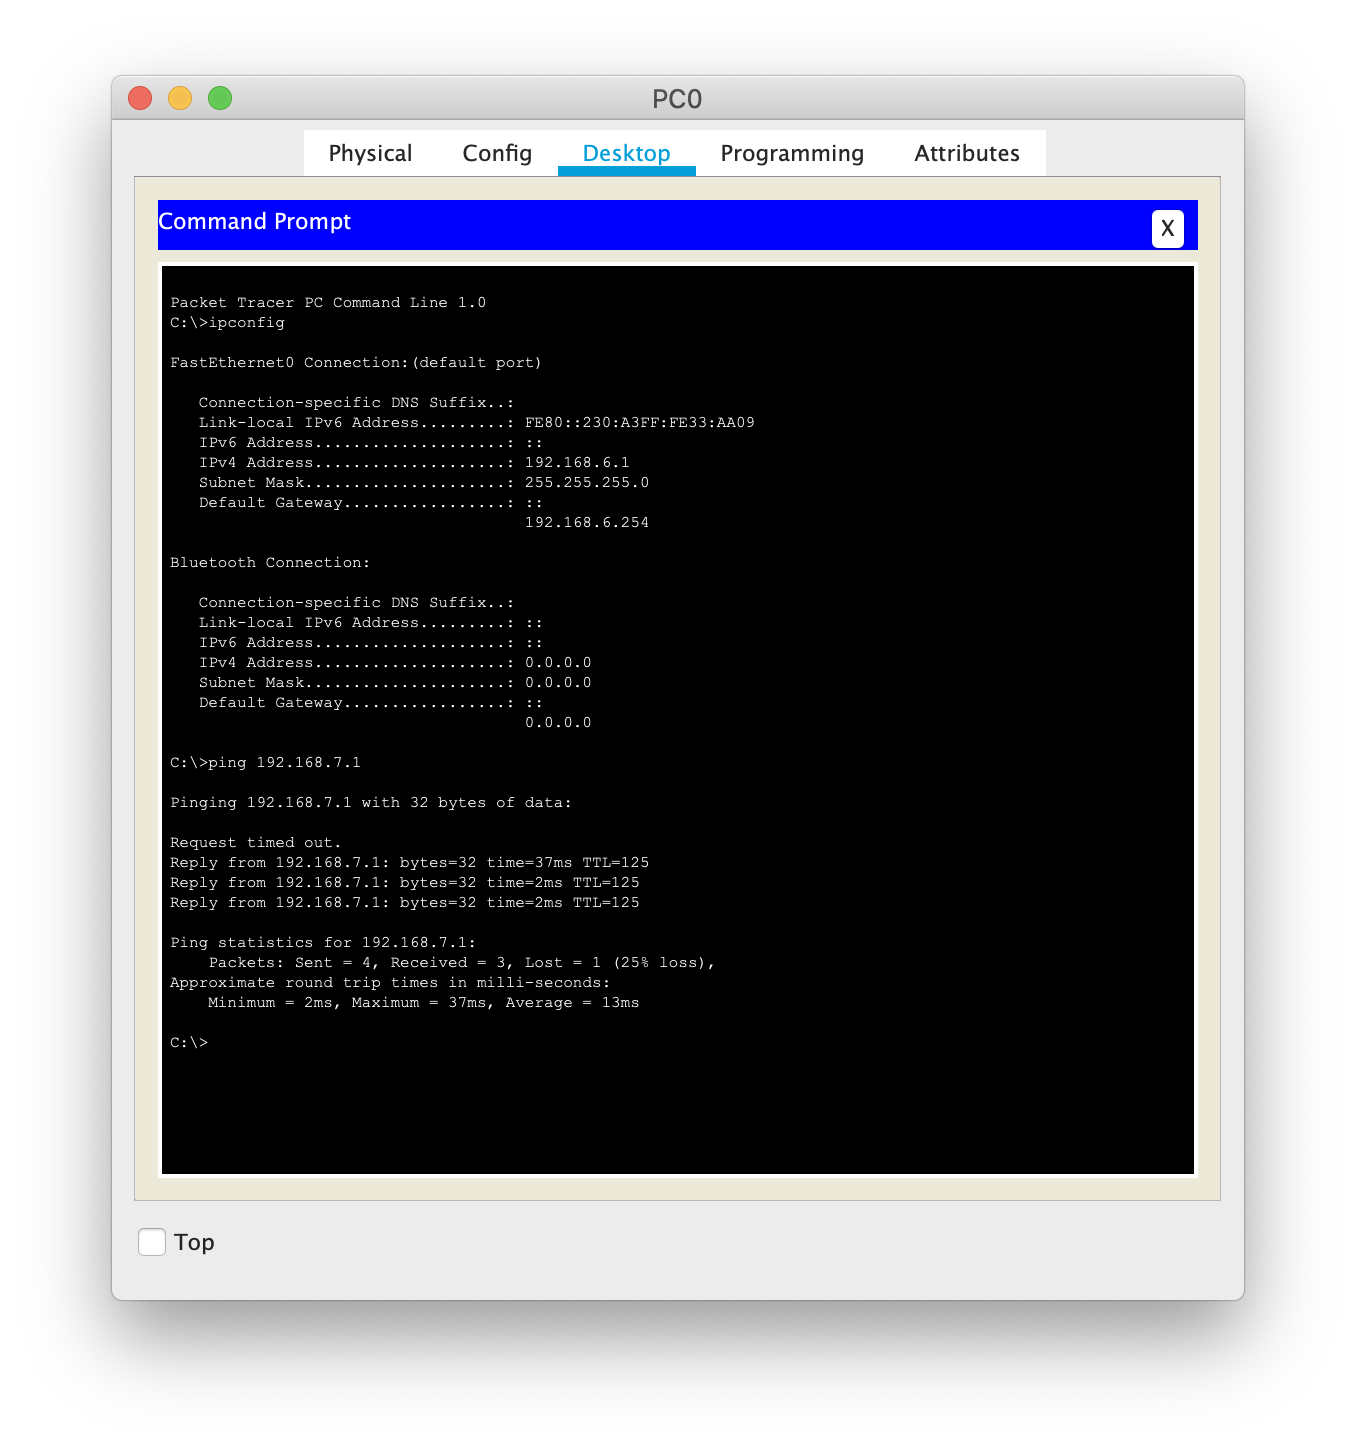
\includegraphics[width=0.495\linewidth]{inc/img/ping-0-3.png}
	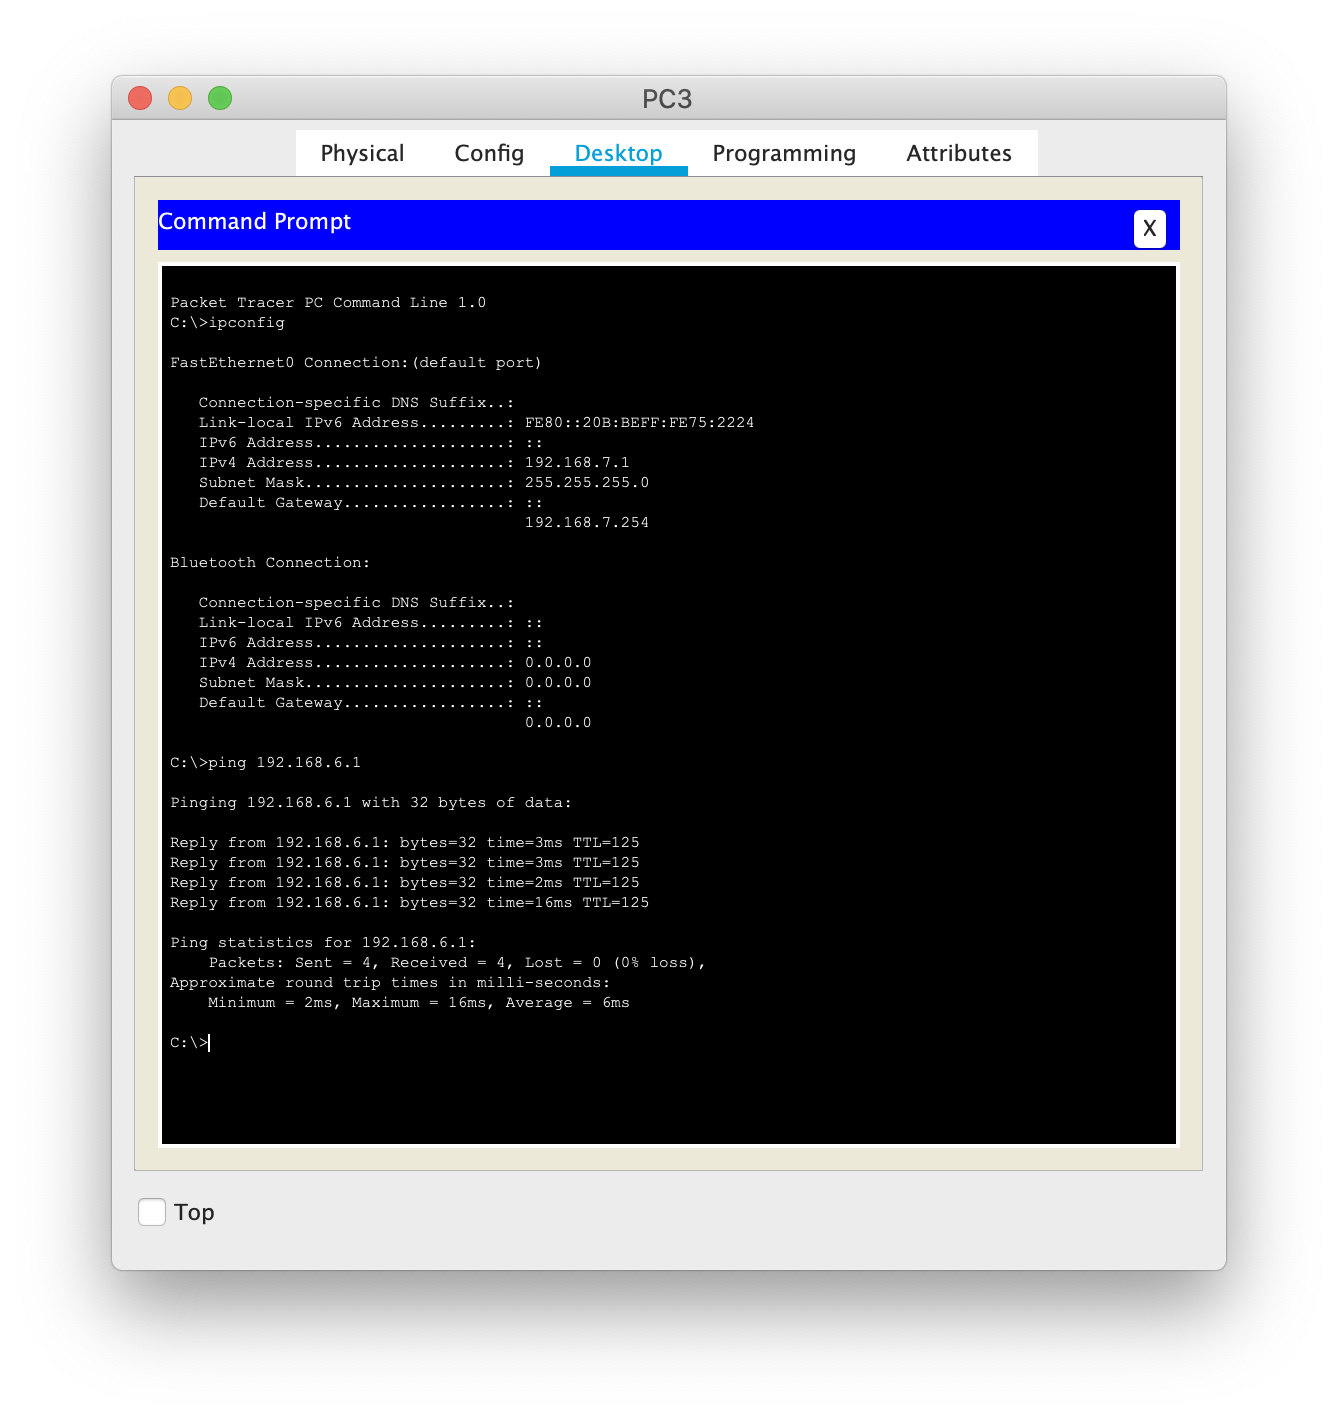
\includegraphics[width=0.495\linewidth]{inc/img/ping-3-0.png}
	\caption{Пинги между PC0 и PC3}
\end{figure}

\chapter{Задание 3}

Настроить динамическую маршрутизацию в сети в прилагаемом .pkt файле на стенде II через протокол OSPF так, чтобы пинг любым хостом или маршрутизатором любого другого хоста или маршрутизатора был успешным.
Разделить при этом сеть на области OSPF в соответствии со схемой.
Выполнить указания в лабораторной работе.
Представить отдельным .pkt файлом.

\section{Настройка}

\begin{lstlisting}[gobble=8, caption=Настройка маршрутизатора Router7]
	Router>en
	Router#sh ip ospf interface

	Router#conf t
	Router(config)#route ospf 1
	Router(config-router)#network 192.168.6.0 0.0.0.255 area 1
	Router(config-router)#network 192.168.16.0 0.0.0.255 area 0
	Router(config-router)#ex
	Router(config)#in G 0/0/0
	Router(config-if)#ip ospf authentication-key key
	Router(config-if)#ex
	Router(config)#in G 0/0/1
	Router(config-if)#ip ospf authentication-key key
	Router(config-if)#ex
	Router(config)#ex
	Router#ex
\end{lstlisting}

\begin{lstlisting}[gobble=8, caption=Настройка маршрутизатора Router8]
	Router>en
	Router#sh ip ospf interface

	Router#conf t
	Router(config)#route ospf 1
	Router(config-router)#network 192.168.7.0 0.0.0.255 area 2
	Router(config-router)#network 192.168.16.0 0.0.0.255 area 0
	Router(config-router)#ex
	Router(config)#in G 0/0/0
	Router(config-if)#ip ospf authentication-key key
	Router(config-if)#ex
	Router(config)#in G 0/0/1
	Router(config-if)#ip ospf authentication-key key
	Router(config-if)#ex
	Router(config)#ex
	Router#ex
\end{lstlisting}

\begin{lstlisting}[gobble=8, caption=Настройка маршрутизатора Router9]
	Router>en
	Router#sh ip ospf interface

	Router#conf t
	Router(config)#route ospf 1
	Router(config-router)#network 192.168.8.0 0.0.0.255 area 3
	Router(config-router)#network 192.168.16.0 0.0.0.255 area 0
	Router(config-router)#ex
	Router(config)#in G 0/0/0
	Router(config-if)#ip ospf authentication-key key
	Router(config-if)#ex
	Router(config)#in G 0/0/1
	Router(config-if)#ip ospf authentication-key key
	Router(config-if)#ex
	Router(config)#ex
	Router#ex
\end{lstlisting}

\begin{lstlisting}[gobble=8, caption=Настройка маршрутизатора Router10]
	Router>en
	Router#sh ip ospf interface

	Router#conf t
	Router(config)#route ospf 1
	Router(config-router)#network 192.168.9.0 0.0.0.255 area 4
	Router(config-router)#network 192.168.16.0 0.0.0.255 area 0
	Router(config-router)#ex
	Router(config)#in G 0/0/0
	Router(config-if)#ip ospf authentication-key key
	Router(config-if)#ex
	Router(config)#in G 0/0/1
	Router(config-if)#ip ospf authentication-key key
	Router(config-if)#ex
	Router(config)#ex
	Router#ex
\end{lstlisting}

\section{Проверка}

\begin{lstlisting}[gobble=8, caption=\code{Router7\# show ip route}]
	Router>en
	Router#sh ip ro
	Codes: L - local, C - connected, S - static, R - RIP, M - mobile, B - BGP
	D - EIGRP, EX - EIGRP external, O - OSPF, IA - OSPF inter area
	N1 - OSPF NSSA external type 1, N2 - OSPF NSSA external type 2
	E1 - OSPF external type 1, E2 - OSPF external type 2, E - EGP
	i - IS-IS, L1 - IS-IS level-1, L2 - IS-IS level-2, ia - IS-IS inter area
	* - candidate default, U - per-user static route, o - ODR
	P - periodic downloaded static route

	Gateway of last resort is not set

	192.168.6.0/24 is variably subnetted, 2 subnets, 2 masks
	C       192.168.6.0/24 is directly connected, GigabitEthernet0/0/0
	L       192.168.6.254/32 is directly connected, GigabitEthernet0/0/0
	O IA 192.168.7.0/24 [110/2] via 192.168.16.253, 00:27:05, GigabitEthernet0/0/1
	O IA 192.168.8.0/24 [110/2] via 192.168.16.252, 00:27:05, GigabitEthernet0/0/1
	O IA 192.168.9.0/24 [110/2] via 192.168.16.251, 00:27:05, GigabitEthernet0/0/1
	192.168.16.0/24 is variably subnetted, 2 subnets, 2 masks
	C       192.168.16.0/24 is directly connected, GigabitEthernet0/0/1
	L       192.168.16.254/32 is directly connected, GigabitEthernet0/0/1

	Router#ex
\end{lstlisting}

\begin{figure}[H]
	\centering
	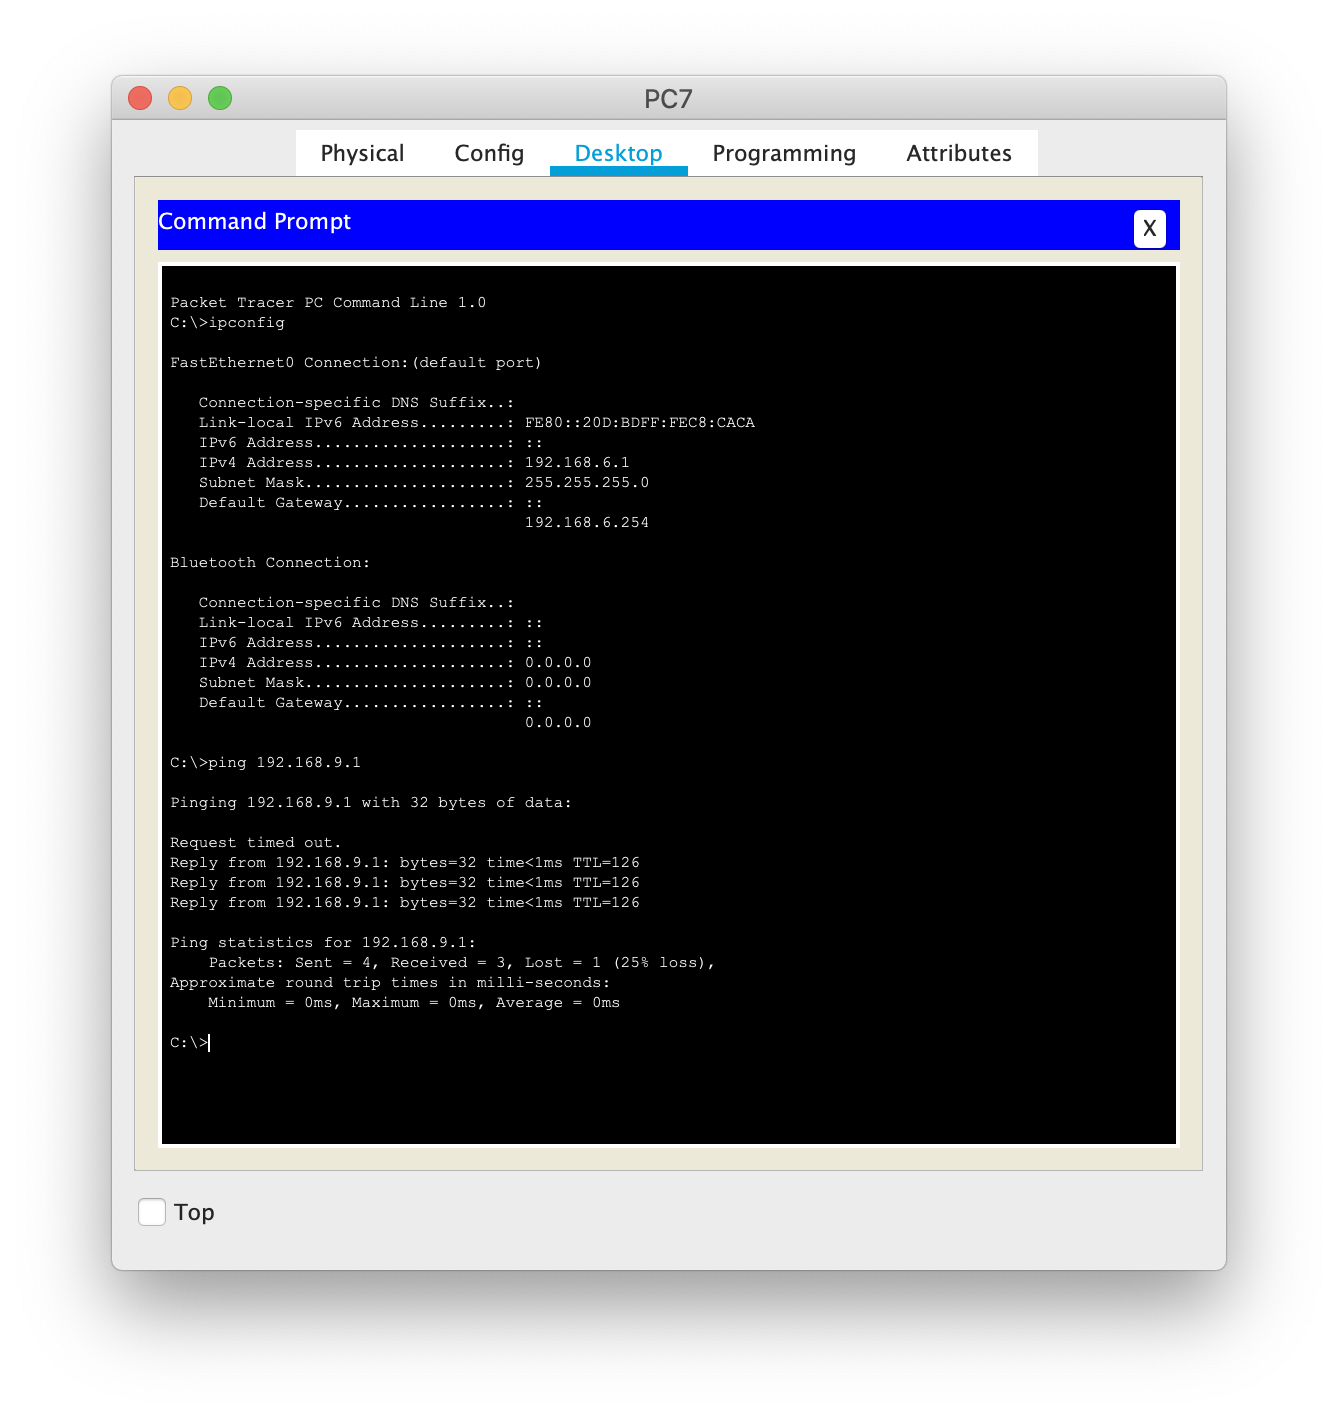
\includegraphics[width=0.495\linewidth]{inc/img/ping-7-10.png}
	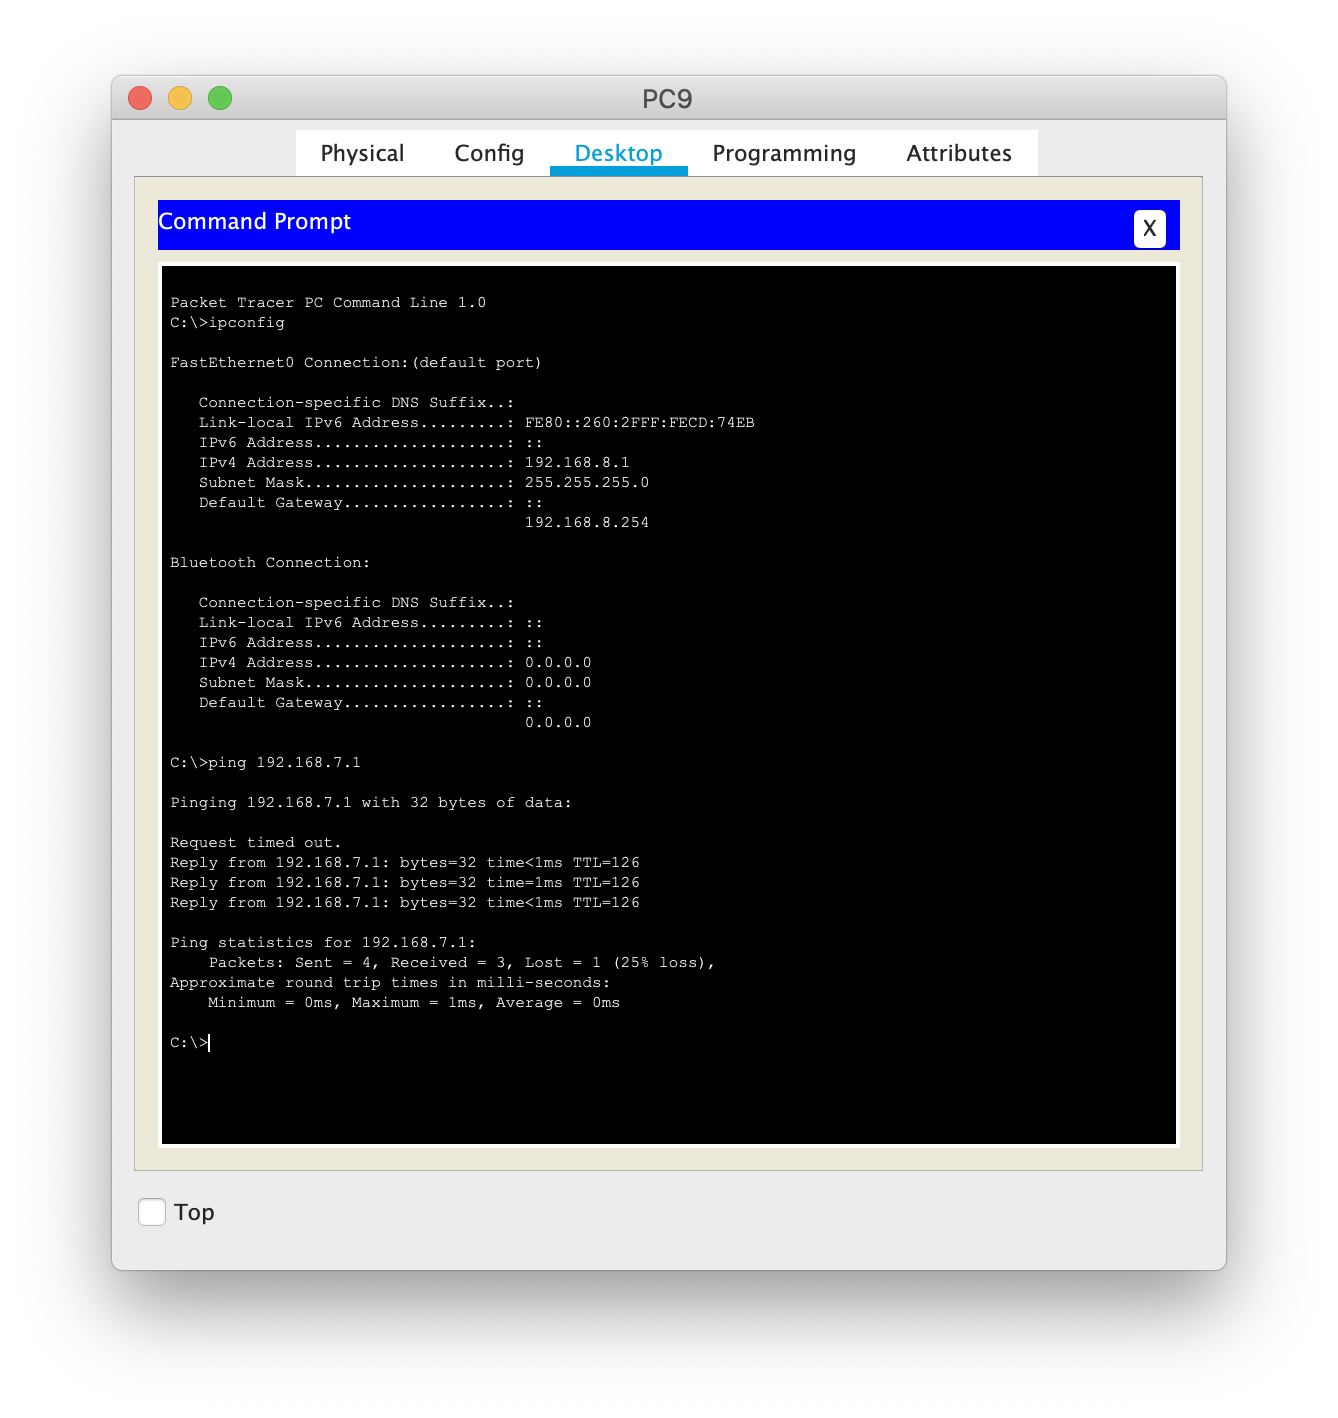
\includegraphics[width=0.495\linewidth]{inc/img/ping-9-8.png}
	\caption{Пинги между (PC7 и PC10) и (PC9 и PC8)}
\end{figure}

\begin{lstlisting}[gobble=8, caption=\code{Router7\# show ip ospf neighbor}]
	Router>en
	Router#sh ip ospf neighbor
	Neighbor ID     Pri   State           Dead Time   Address         Interface
	192.168.16.251    1   FULL/DROTHER    00:00:37    192.168.16.251  GigabitEthernet0/0/1
	192.168.16.252    1   FULL/DROTHER    00:00:37    192.168.16.252  GigabitEthernet0/0/1
	192.168.16.253    1   FULL/BDR        00:00:37    192.168.16.253  GigabitEthernet0/0/1
	Router#ex
\end{lstlisting}

\begin{lstlisting}[gobble=8, caption=\code{Router8\#  show ip ospf neighbor}]
	Router>en
	Router#sh ip ospf neighbor
	Neighbor ID     Pri   State           Dead Time   Address         Interface
	192.168.16.251    1   FULL/DROTHER    00:00:31    192.168.16.251  GigabitEthernet0/0/1
	192.168.16.252    1   FULL/DROTHER    00:00:31    192.168.16.252  GigabitEthernet0/0/1
	192.168.16.254    1   FULL/DR         00:00:31    192.168.16.254  GigabitEthernet0/0/1
	Router#ex
\end{lstlisting}

\begin{lstlisting}[gobble=8, caption=\code{Router9\# show ip ospf neighbor}]
	Router>en
	Router#sh ip ospf neighbor
	Neighbor ID     Pri   State           Dead Time   Address         Interface
	192.168.16.251    1   2WAY/DROTHER    00:00:35    192.168.16.251  GigabitEthernet0/0/1
	192.168.16.253    1   FULL/BDR        00:00:36    192.168.16.253  GigabitEthernet0/0/1
	192.168.16.254    1   FULL/DR         00:00:35    192.168.16.254  GigabitEthernet0/0/1
	Router#ex
\end{lstlisting}

\begin{lstlisting}[gobble=8, caption=\code{Router10\#  show ip ospf neighbor}]
	Router>en
	Router#sh ip ospf neighbor
	Neighbor ID     Pri   State           Dead Time   Address         Interface
	192.168.16.252    1   2WAY/DROTHER    00:00:31    192.168.16.252  GigabitEthernet0/0/1
	192.168.16.253    1   FULL/BDR        00:00:31    192.168.16.253  GigabitEthernet0/0/1
	192.168.16.254    1   FULL/DR         00:00:30    192.168.16.254  GigabitEthernet0/0/1
	Router#ex
\end{lstlisting}

Router7 — DR.
Router8 — BDR.
Все маршрутизаторы являются пограничными.

\end{document}
